% Copyright (c) 2022 by Lars Spreng
% This work is licensed under the Creative Commons Attribution 4.0 International License. 
% To view a copy of this license, visit http://creativecommons.org/licenses/by/4.0/ or send a letter to Creative Commons, PO Box 1866, Mountain View, CA 94042, USA.

%~~~~~~~~~~~~~~~~~~~~~~~~~~~~~~~~~~~~~~~~~~~~~~~~~~~~~~~~~~~~~~~~~~~~~~~~~~~~~~
% You can add your packages and commands to the loadslides.tex file. 
% The files in the folder "styles" can be modified to change the layout and design of your slides.
% I have included examples on how to use the template below. 
% Some of these examples are taken from the Metropolis template.
%~~~~~~~~~~~~~~~~~~~~~~~~~~~~~~~~~~~~~~~~~~~~~~~~~~~~~~~~~~~~~~~~~~~~~~~~~~~~~~


\documentclass[11pt,notheorems,hyperref={pdfauthor=whatever}]{beamer}


% Copyright (c) 2022 by Lars Spreng
% This work is licensed under the Creative Commons Attribution 4.0 International License. 
% To view a copy of this license, visit http://creativecommons.org/licenses/by/4.0/ or send a letter to Creative Commons, PO Box 1866, Mountain View, CA 94042, USA.

%~~~~~~~~~~~~~~~~~~~~~~~~~~~~~~~~~~~~~~~~~~~~~~~~~~~~~~~~~~~~~~~~~~~~~~~~~~~~~~
% Add your packages and commands to this file
%~~~~~~~~~~~~~~~~~~~~~~~~~~~~~~~~~~~~~~~~~~~~~~~~~~~~~~~~~~~~~~~~~~~~~~~~~~~~~~
\usepackage{xcolor}
\usepackage{tikz-cd}

%~~~~~~~~~~~~~~~~~~~~~~~~~~~~~~~~~~~~~~~~~~~~~~~~~~~~~~~~~~~~~~~~~~~~~~~~~~~~~~
% Fonts
% \RequirePackage{palatino} % for serif slides
% \usefonttheme{serif}
\RequirePackage[scaled]{helvet} % for sans-serif slides

\RequirePackage[utf8]{inputenc}
\RequirePackage[T1]{fontenc}


\usepackage{styles/elegantmacros}
\usefolder{styles}
\usetheme[style=gold]{elegant}

\newcommand{\makepart}[1]{ % For convenience
\part{#1} \frame{\partpage}
}

%~~~~~~~~~~~~~~~~~~~~~~~~~~~~~~~~~~~~~~~~~~~~~~~~~~~~~~~~~~~~~~~~~~~~~~~~~~~~~~

%~~~~~~~~~~~~~~~~~~~~~~~~~~~~~~~~~~~~~~~~~~~~~~~~~~~~~~~~~~~~~~~~~~~~~~~~~~~~~~
% Figures
\RequirePackage{booktabs}
\RequirePackage{colortbl}
\RequirePackage{ragged2e}
\RequirePackage{schemabloc}
%\RequirePackage{natbib}
\RequirePackage{caption}
\RequirePackage{subcaption}
\RequirePackage{tabularx}
\RequirePackage{array}
\RequirePackage{multirow}
\RequirePackage[%
  natbib=true, backend=biber,%
  style=apa, isbn=false,url=false,uniquename=false%, useprefix=true%
  ]{biblatex}
\addbibresource{references.bib}
\newcolumntype{Y}{>{\centering\arraybackslash}X}

%~~~~~~~~~~~~~~~~~~~~~~~~~~~~~~~~~~~~~~~~~~~~~~~~~~~~~~~~~~~~~~~~~~~~~~~~~~~~~~

%~~~~~~~~~~~~~~~~~~~~~~~~~~~~~~~~~~~~~~~~~~~~~~~~~~~~~~~~~~~~~~~~~~~~~~~~~~~~~~
% Figures
\RequirePackage{wrapfig}
\RequirePackage{pgfplots}
\RequirePackage{graphicx}
\RequirePackage{adjustbox}
\RequirePackage{environ}
\pgfplotsset{compat=1.18}

\makeatletter
\newsavebox{\measure@tikzpicture}
\NewEnviron{scaletikzpicturetowidth}[1]{%
  \def\tikz@width{#1}%
  \def\tikzscale{1}\begin{lrbox}{\measure@tikzpicture}%
  \BODY
  \end{lrbox}%
  \pgfmathparse{#1/\wd\measure@tikzpicture}%
  \edef\tikzscale{\pgfmathresult}%
  \BODY
}
\makeatother
%~~~~~~~~~~~~~~~~~~~~~~~~~~~~~~~~~~~~~~~~~~~~~~~~~~~~~~~~~~~~~~~~~~~~~~~~~~~~~~

%~~~~~~~~~~~~~~~~~~~~~~~~~~~~~~~~~~~~~~~~~~~~~~~~~~~~~~~~~~~~~~~~~~~~~~~~~~~~~~
% Maths 
\RequirePackage{textcomp}
\RequirePackage{amsmath} 
\RequirePackage{amsthm}
\RequirePackage{mathtools}
%\RequirePackage{bbm}
%\RequirePackage{algorithm}
%\RequirePackage[osf,sc]{mathpazo}
%\RequirePackage{pifont}
%\newcommand{\xmark}{\ding{55}}%
%\numberwithin{equation}{section}
\DeclareMathOperator*{\argmax}{arg\,max}
\DeclareMathOperator*{\argmin}{arg\,min}

\setbeamertemplate{theorems}[numbered] % to number

\theoremstyle{definition}
\newtheorem{fact}{Fact}[section]
\newtheorem{examp}{Example}[section]

\theoremstyle{plain}
\newtheorem{definition}{Definition}[section]
\newtheorem{proposition}{Proposition}
\newtheorem{theorem}{Theorem}
\newtheorem{assumption}{Assumption}

\providecommand{\H}{\mathscr{H}}      
\providecommand{\E}{\mathbb{E}}
\makeatletter
\def\munderbar#1{\underline{\sbox\tw@{$#1$}\dp\tw@\z@\box\tw@}}
\makeatother

%~~~~~~~~~~~~~~~~~~~~~~~~~~~~~~~~~~~~~~~~~~~~~~~~~~~~~~~~~~~~~~~~~~~~~~~~~~~~~~
 % Loads packages and some defined commands

\addbibresource{../references/references.bib}

\title[
% Text entered here will appear in the bottom middle
]{Brief Introduction to Number Theoretic Transform}

\subtitle{From the Perspective of Ring Theory}

\author[
% Text entered here will appear in the bottom left corner
]{
    Cesare Huang Cheng Wei
}

\institute{Academia Sinica}
\date{January 8, 2025}

\begin{document}

% Generate title page
{
\setbeamertemplate{footline}{} 
\begin{frame}
  \titlepage
\end{frame}
}
\addtocounter{framenumber}{-1}

% You can declare different parts as a parentof sections
\begin{frame}{Table of Contents}
    \tableofcontents
\end{frame}


\section{Introduction and Goal}

\begin{frame}{Motivation and Goals}
  \begin{itemize}
    \item<1-> \textbf{Core Problem}: Fast polynomial multiplication in 
          \(\mathbb{Z}_{p}[x]/(x^n - 1)\), where \(n\) is a power of 2.\\
          The problems we deal with include more general quotient rings, 
          but in this slide, we firstly focus on such simple ring 
          for the purpose of illustration.
    \item<2-> \textbf{Background}:
          \begin{itemize}
            \item In many applications in cryptography, we have to multiply the elements
                  in the ring of the kind \(\mathbb{Z}_{p}[x]/(x^n - 1)\), 
                  which is a very time-consuming operation.
            \item Suppose we can perform such operation more efficiently, 
                  then in the same cost of computational resource (i.e., time),
                  we can perform such multiplication for larger \(n\), 
                  and thus improve the security level of the cryptographic scheme.
          \end{itemize}
  \end{itemize}
\end{frame}


\section{Residual Number System and Theory of Quotient Rings}

\begin{frame}
    \begin{itemize}
        \item <1->We first take a step back to deal with the multiplication in 
              the ring \(\mathbb{Z}/ n\mathbb{Z}\).
        \item <2->For example, let's consider the toy example of multiplication 
              in the ring \(\mathbb{Z}/ 105\mathbb{Z}\).
        \item <3->Note that \( 105 = 3 \cdot 5\cdot 7\), 
              and the factors are co-prime (ideals), 
              so we have the following decomposition:
              \[ \mathbb{Z}/ 105\mathbb{Z} \cong 
                 \mathbb{Z}/ 3\mathbb{Z} \times 
                 \mathbb{Z}/ 5\mathbb{Z} \times 
                 \mathbb{Z}/ 7\mathbb{Z} \]
        \item <4->Suppose we want to perform the multiplication \(31 * 27 = 102\) in 
        \item <5->Suppose we want to perform the multiplication \(31 * 27 = 102\) in 
              the ring \(\mathbb{Z}/ 105\mathbb{Z}\)
        \item <6->We first project the operands (31, 27) to the three "coordinate"-rings:
              \[ 31 \mapsto (1, 1, 3) \quad 27 \mapsto (0, 2, 6) \]
        \item <7->Multiply the corresponding "coordinates" to get
              \[ (1, 1, 3) \cdot (0, 2, 6) = (0, 2, 4) \]
        \item <8->Finally, we recombine the result to get the final answer:
              The process involves the so-called Chinese Remainder Theorem (CRT),
              that is, to find the solution to the system
              \[
                x \equiv 0 \pmod{3}, \quad
                x \equiv 2 \pmod{5}, \quad
                x \equiv 4 \pmod{7}
              \]
              The solution is \(x = 102\), 
              which is the answer to the original multiplication.
             

    \end{itemize}
\end{frame}


\begin{frame}{Remarks on CRT}
    \begin{itemize}
        \item <1->Some may argue that the final recombination step is even costly. 
              However, there exists some efficient algorithms to perform the CRT. 
        \item <2->Another advantage of the RNS CRT approach is that, after decomposing 
              the ring into several "coordinate"-rings, we can perform the 
              multiplication in the "coordinate"-rings in parallel. 
        \item <3->If the whole process involves many times of multiplication, 
              we can leave the big integers in the RNS coordinate representations, 
              and after performing all required multiplications, 
              recombine the results via the CRT once.
        \item <4->Such technique is applicable in real-world, for example, 
              to compute a discrete logarithm in the ring \(\mathbb{Z}/ n\mathbb{Z}\).
        \item <5->For more discussion on the RNS, see the paper: 
        Modular exponentiation via the explicit Chinese remainder theorem
        by DJB.

    \end{itemize}
\end{frame}





\subsection{Quotient Rings}
\begin{frame}
    \begin{itemize}
        \item <1->So far, we have seen many notations like 
            \[ \mathbb{Z}/ n\mathbb{Z}, \quad \mathbb{Z}[x]/(x^n - 1), \quad \mathbb{Z}_{p}[x]/(x^n - 1)  \]
        \item <2->These are examples of quotient rings. 
        \item <3->The meaning of \( \mathbb{Z}/n\mathbb{Z} \) is familiar to us, 
              it means that all operations are performed modulo \(n\).
        \item <4->We can extend the idea to polynomial operations: 
              \begin{itemize}
                   \item the set \( \mathbb{Z}[x] \) is the set of all polynomials 
                         with integer coefficients. 
                         Operations are performed as usual.
                   \item the set \( \mathbb{Z}[x]/(x^n - 1) \) thus meanes that 
                         all operations are performed modulo \(x^n - 1\).
                   \item For example, in the ring \( \mathbb{Z}[x]/(x^2 - 1) \), 
                       \[ (x + 1) \cdot (x + 2) = x^2 + 3x + 2 \equiv 3x + 4 \pmod{x^2 - 1} \]
              \end{itemize}
 
        \item <5->Generally, \(\mathbb{Z}[x]/(f(x))\): Polynomial congruences where \(f(x) \equiv 0\).
        \item <6->We also write the quotient integer rings \(\mathbb{Z} / n\mathbb{Z}\) as \(\mathbb{Z}_n\)
        \item <7->Hence, the meaning of \(\mathbb{Z}_{p}[x]/(x^n - 1)\) 
              is that the coefficients are reduced modulo \(p\),
              and the polynomial is reduced modulo \(x^n - 1\).
  \end{itemize}
\end{frame}


\subsection{Decomposition of \( \mathbb{Z}[x]/(x^2-1) \)}
\begin{frame}
\begin{itemize}
    \item <1->From the experience of the RNS, we now try the same trick on the problem of 
          multiplication in the ring \( \mathbb{Z}[x]/(x^2 - 1) \).
    \item <2->Easy to see that \(x^2 - 1 = (x - 1)(x + 1)\), 
          and the factors are co-prime (ideals),
          so we have the following decomposition:
          \[ \mathbb{Z}[x]/(x^2 - 1) \cong 
             \mathbb{Z}[x]/(x - 1) \times 
             \mathbb{Z}[x]/(x + 1) \]
    \item <3->Suppose we want to multiply \( (3 + 1x) \cdot (2 + 7x) = 13 + 23x\) in the ring 
          \( \mathbb{Z}[x]/(x^2 - 1) \).
    \item <4->We first project the operands to the two "coordinate"-rings:
          \[
            3+1x \mapsto (4,2),\quad 2+7x \mapsto (9,-5).
          \]
    \item <5->Multiply the corresponding "coordinates" to get
        \[
            (4,2)\cdot (9,-5) = (36,-10).
        \]
    \item <6->Finally, we recombine the result to the final asnwer: 
          that is, to find the solution to the system
          \[
            f(x) \equiv 36 \pmod{x-1},\quad 
            f(x) \equiv -10 \pmod{x+1}.
          \]
          The solution is \(f(x) = 13 + 23 x\).
        \item <7->It seems that the recombination is very hard to solve. But, no, see the next slide.
  \end{itemize}
\end{frame}

\begin{frame}
    \begin{itemize}
        \item <1->A saying goes that "How to go forward then how to go back" (Cesare Huang, 2024)
        \item <2->Let \(a + b x\) be one of the operand in the ring \( \mathbb{Z}[x]/ (x^{2}-1)\),
            then we have the following projection:
            \begin{align*}
                \mathbb{Z}[x] / (x^{2}-1) &\cong 
                \mathbb{Z}[x] / (x-1) \times 
                \mathbb{Z}[x] / (x+1)  \\
                a + b x &\mapsto (a+b, a-b)\\
                \frac{A+B}{2} + \frac{A-B}{2}x &\mapsto (A,B).
            \end{align*}

        \item <3->Hence, the recombination is easy, once receive the \(A,B\) from the component-wise multiplication, 
              the solution in \( \mathbb{Z}[x] / (x^{2} - 1) \) is simply
              \[
                \frac{A+B}{2} + \frac{A-B}{2}x
              \]

        \item <4->Check:
          \[
            f(x) \equiv 36 \pmod{x-1},\quad 
            f(x) \equiv -10 \pmod{x+1}.
          \]
          The solution is \(f(x) = 13 + 23 x\).
    \end{itemize}
\end{frame}

\begin{frame}
    \begin{itemize}
        \item <1->Let's now give a full analysis on the fast multiplication 
            in the ring \( \mathbb{Z}[x] / (x^{2} - 1) \) just invented.
        \item <2->Let \( a + b x \) and \( c + d x \) be the two operands, 
            out algorithm goes as follows:
            \begin{enumerate}
                \item <3->Project the ring elements into two "coordinate"-rings:
                    \[
                        a + b x \mapsto (a+b, a-b),\quad c + d x \mapsto (c+d, c-d).
                    \]
                    It takes four add/sub operations in this step.
                \item <4->Multiply the "coordinates" to get
                    \[
                        (a+b, a-b) \cdot (c+d, c-d) = ((a+b)(c+d), (a-b)(c-d)) := (A,B).
                    \]
                    It takes two multiplications in this step.

                \item <5->Recombine the result to get the final answer:
                    \[
                        \frac{A+B}{2} + \frac{A-B}{2}x.
                    \]
                    It takes two add/sub operations and two divided by 2 operations in this step.
                    Note that divided by 2 is a shift operation, which is very fast.
            \end{enumerate}
    \end{itemize}
\end{frame}

\begin{frame}
    \begin{itemize}
        \item <1->The algorithm we just invented takes:
            \begin{itemize}
                \item 6 add/sub operations
                \item 2 multiplications
                \item 2 shift operation
            \end{itemize}
        \item <2->The naive algorithm (schoolbook multiplication) takes:
            \begin{itemize}
                \item 4 multiplications
                \item 2 additions
            \end{itemize}
        \item <3->The analysis we just made are based on number of mathematic operations.
            This is illustrative, but not the whole story.
            In practice, please benchmark the performance by the actual cycle-count.
    \end{itemize}
\end{frame}


\subsection{Decomposition of \( \mathbb{Z}[x]/(x^4-1) \)}

\begin{frame}
    \begin{itemize}
        \item <1->After experience the fast multiplication brought by the decomposition of 
            \( \mathbb{Z}[x]/(x^{2}-1) \), we now try to decompose the ring 
            \( \mathbb{Z}[x]/(x^{4}-1) \).
        \item <2->Easy to see that \(x^{4}-1 = (x^{2}-1)(x^2+1)\), 
            and the factors are co-prime (ideals),
            so we have the following decomposition:
            \[ \mathbb{Z}[x]/(x^4 - 1) \cong 
            \mathbb{Z}[x]/(x^2 - 1) \times 
            \mathbb{Z}[x]/(x^2 + 1) \]
        \item <3->Until here, we can already develop a fast multiplication algorithm by such decomposition.
            But it the first coordinate-ring can be further decomposed,
            and it seems that decomposing then one more time can bring more speedup.
        \item <4->The first ring can be decomposed as we just did.
            However, for the second one,
            \[ \mathbb{Z}[x]/(x^2 + 1) \]
            there is no obvious factorization of \(x^2 + 1\).
        \item <5->One way is to employ the complex number field, 
            and we have the following decomposition:
            \[ \mathbb{Z}[x]/(x^2 + 1) \cong 
            \mathbb{Z}[x]/(x - i) \times 
            \mathbb{Z}[x]/(x + i) \]
            The same trick as above can be applied in the cost of introducing complex numbers.
            Such trick is called the Discrete Fourier Transform (DFT).
        \item <6->The concept of the Number Theoretic Transform (NTT) is similar to DFT, 
            but required more well-strucutred ring.
    \end{itemize}
\end{frame}

\begin{frame}
    \begin{itemize}
        \item <1->One way is to employ the complex number field, 
            and we have the following decomposition:
            \[ \mathbb{Z}[x]/(x^2 + 1) \cong 
            \mathbb{Z}[x]/(x - i) \times 
            \mathbb{Z}[x]/(x + i) \]
        \item <2->The concept of the Number Theoretic Transform (NTT) is similar to DFT, 
            but required more well-strucutred ring.
        \item <3->Recall that our core problem is to deal with the multiplication of
            the ring \( \mathbb{Z}_{p}[x]/(x^{n}-1) \).
            Here, we in particular consider the ring \( \mathbb{Z}_{p}[x]/(x^{4}-1) \).
        \item <4->The important observation is that, there may be some element in \( \mathbb{Z}_{p}\),
            denoted as \(\omega\), such that \(\omega^{2} = -1\), which, serves as the imaginary unit
            as in the DFT.

        \item <5->Take, for example, the ring \( \mathbb{Z}_{17}[x]/(x^{4}-1)\) for example. 
            In this ring,
            \[
                4^{2} = 16 \equiv -1 \pmod{17}.
            \]
            We thus have the following decomposition:
            \begin{align*}
                \mathbb{Z}_{17}[x]/(x^{2}+1) 
                &= \mathbb{Z}_{17}[x] / (x^{2} - (-1))
                = \mathbb{Z}_{17}[x] / (x^{2} - 4^{2})\\
                &\cong 
                \mathbb{Z}_{17}[x]/(x-4) \times 
                \mathbb{Z}_{17}[x]/(x+4).
            \end{align*}

    \end{itemize}
\end{frame}




\begin{frame}
    \begin{itemize}

        \item <1->Take, for example, the ring \( \mathbb{Z}_{17}[x]/(x^{4}-1)\) for example. 
            In this ring,
            \[
                4^{2} = 16 \equiv -1 \pmod{17}.
            \]
            We thus have the following decomposition:
            \begin{align*}
                \mathbb{Z}_{17}[x]/(x^{2}+1) 
                &= \mathbb{Z}_{17}[x] / (x^{2} - (-1))
                = \mathbb{Z}_{17}[x] / (x^{2} - 4^{2})\\
                &\cong 
                \mathbb{Z}_{17}[x]/(x-4) \times 
                \mathbb{Z}_{17}[x]/(x+4).
            \end{align*}

        \item <2->Hence we have the full decomposition:
            \begin{align*}
                \mathbb{Z}_{17}[x]/(x^{4}-1) 
                &\cong 
                \mathbb{Z}_{17}[x]/(x^{2}-1) \times 
                \mathbb{Z}_{17}[x]/(x^{2}+1)\\
                &\cong 
                \mathbb{Z}_{17}[x]/(x-1) \times 
                \mathbb{Z}_{17}[x]/(x+1) \times 
                \mathbb{Z}_{17}[x]/(x-4) \times 
                \mathbb{Z}_{17}[x]/(x+4).
            \end{align*}

        \item <3->We can analogously develop a fast multiplication algorithm for the ring 
            \( \mathbb{Z}_{17}[x]/(x^{4}-1) \):\\
            projection to coordinate-ring, coordinate-wise multiplication, recombination.
    \end{itemize}
\end{frame}

\begin{frame}
    \begin{itemize}
        \item <4->Suppose we want to multiply two polynomials in the ring \( \mathbb{Z}_{17}[x]/(x^{4}-1) \):
            \[
                3 + 1x + 4x^{2} + 2x^{3},\quad 2 + 7x + 1x^{2} + 2x^{3}.
            \]
        \item The projection goes like:
            \begin{align*}
                \mathbb{Z}_{17}[x]/(x^{4}-1) 
                &\cong 
                \mathbb{Z}_{17}[x]/(x^{2}-1) \times 
                \mathbb{Z}_{17}[x]/(x^{2}+1)\\
                &\cong 
                \mathbb{Z}_{17}[x]/(x-1) \times 
                \mathbb{Z}_{17}[x]/(x+1) \times 
                \mathbb{Z}_{17}[x]/(x-4) \times 
                \mathbb{Z}_{17}[x]/(x+4).\\
                3 + 1x + 4x^{2} + 2x^{3} 
                &\mapsto 
                (7 + 3x, -1 - 1x) \cong (7 + 3x, 16 + 16x),\\
                &\mapsto 
                (10, -4, -5, 3 ) \cong (10, 13, 12, 3)\\
                2 + 7x + 1x^{2} + 2x^{3} 
                &\mapsto 
                (3 + 9x, 1 + 5x)\\
                &\mapsto 
                (12, -6, 21, -19 ) \cong (12, 11, 4, 15).
            \end{align*}
        \item <5->Coordinate-wise multiplication is straightforward:
            \[
                (10, 13, 12, 3) \cdot (12, 11, 4, 15) = (120, 143, 48, 45)
                \cong (1, 7, 14, 11).
            \]
        \item <6->Recombination is not obvious, see the next slide.
    \end{itemize}
\end{frame}


\begin{frame}
    \begin{itemize}
        \item <1->We now try to recombine the result by the information of coordinates
            \[
            (1, 7, 14, 11)\in 
                \mathbb{Z}_{17}[x]/(x-1) \times 
                \mathbb{Z}_{17}[x]/(x+1) \times 
                \mathbb{Z}_{17}[x]/(x-4) \times 
                \mathbb{Z}_{17}[x]/(x+4).
            \]
        \item <2->For the first two coordinate, we can partially recombine them into the ring 
            \( \mathbb{Z}_{17}[x]/(x^{2}-1) \), since they came from the colored projection as shown:
            \begin{align*}
                \mathbb{Z}_{17}[x]/(x^{4}-1) 
                &\cong 
                {\color{blue}\mathbb{Z}_{17}[x]/(x^{2}-1)}\times 
                \mathbb{Z}_{17}[x]/(x^{2}+1)\\
                &\cong 
                {\color{blue}\mathbb{Z}_{17}[x]/(x-1)} \times 
                {\color{blue}\mathbb{Z}_{17}[x]/(x+1)} \times 
                \mathbb{Z}_{17}[x]/(x-4) \times 
                \mathbb{Z}_{17}[x]/(x+4).
            \end{align*}
        \item <3->Such partial recombination is easy, as we done before:
            \[
                4 - 3x = \frac{1+7}{2} + \frac{1-7}{2}x .
            \]

    \end{itemize}
\end{frame}


\begin{frame}
    \begin{itemize}
        \item <1->We now try to recombine the result, denoted \(f(x)\), by the information of coordinates
            \[
            (1, 7, 14, 11)\in 
                \mathbb{Z}_{17}[x]/(x-1) \times 
                \mathbb{Z}_{17}[x]/(x+1) \times 
                \mathbb{Z}_{17}[x]/(x-4) \times 
                \mathbb{Z}_{17}[x]/(x+4).
            \]
        \item <2->For the last two coordinate, we can partially recombine them into the ring 
            \( \mathbb{Z}_{17}[x]/(x^{2}-1) \), since they came from the colored projection as shown:
            \begin{align*}
                \mathbb{Z}_{17}[x]/(x^{4}-1) 
                &\cong 
                \mathbb{Z}_{17}[x]/(x^{2}-1)\times 
                {\color{red}\mathbb{Z}_{17}[x]/(x^{2}+1)}\\
                &\cong 
                \mathbb{Z}_{17}[x]/(x-1) \times 
                \mathbb{Z}_{17}[x]/(x+1) \times 
                {\color{red}\mathbb{Z}_{17}[x]/(x-4)} \times 
                {\color{red}\mathbb{Z}_{17}[x]/(x+4)}.
            \end{align*}
        \item <3->But such partial recombination is a little bit tricky,
            \begin{align*}
                \mathbb{Z}_{17}[x] / (x^{2}+1) &\cong 
                \mathbb{Z}_{17}[x] / (x - 4) \times
                \mathbb{Z}_{17}[x] / (x + 4) \\
                a + bx &\mapsto (a+4b, a-4b) = (A,B).\\
                \frac{1}{2}(A+B) + \frac{1}{2}\frac{A-B}{4}x &\mapsto (A,B).
            \end{align*}
        \item <4->In this case, the recombination goes:
            \[
                \frac{1}{2}(14+11) + \frac{1}{2}\frac{14-11}{4}x = 4 + 11x.
            \]
            Note that the division are performed in the ring \( \mathbb{Z}_{17} \).
        \item Check that \( 4 + 11x \) projects to \( (14, 11)\).
    \end{itemize}
\end{frame}


\begin{frame}
    \begin{itemize}
        \item <1->So far, we know that the answer of the multiplication, denoted \(f(x)\), 
            represented in the first layer of decomposition is:
            \begin{align*}
                \mathbb{Z}_{17}[x] / (x^{4} - 1) &\cong
                \mathbb{Z}_{17}[x] / (x^2-1) \times 
                \mathbb{Z}_{17}[x] / (x^2+1) \\
                f(x) &\mapsto (4 - 3x, 4 + 11x)\\
            \end{align*}
            We have to do one more layer of recombination to get the final answer.

        \item <2->Take a look at the first layer of decomposition:
            \begin{align*}
                \mathbb{Z}_{17}[x] / (x^{4} - 1) &\cong
                \mathbb{Z}_{17}[x] / (x^2-1) \times
                \mathbb{Z}_{17}[x] / (x^2+1) \\
                (a_{0} + a_{1}x + a_{2}x^{2} + a_{3}x^{3}) &\mapsto
                (a_{0} + a_{2} + (a_{1} + a_{3})x, 
                a_{0} - a_{2} + (a_{1} - a_{3})x) := (A_{0} + A_{1}x, A_{2} + A_{3}x).
            \end{align*}
            Hence
            \[
                \frac{1}{2}(A_{0} + A_{2})  + 
                \frac{1}{2}(A_{1} + A_{3})x +
                \frac{1}{2}(A_{0} - A_{2})x^{2} +
                \frac{1}{2}(A_{1} - A_{3})x^{3} \mapsto
                (A_{0} + A_{1}x, A_{2} + A_{3}x).
            \]

        \item <3->Apply to our case, the final answer is:
            \[
                \frac{1}{2}(4 + 4) + \frac{1}{2}(-3 + 11)x + 
                \frac{1}{2}(4 - 4)x^{2} + \frac{1}{2}(-3 - 11)x^{3} = 4 + 4x + 0x^{2} - 7x^{3}.
            \]
        \item Check that \(f(x) = 4 + 4x + 0x^{2} - 7x^{3}\) projects to \( (1, 7, 14, 11)\).
    \end{itemize}
\end{frame}

\begin{frame}
    \begin{itemize}
        \item <1->Let's now give a summary of the fast multiplication algorithm just invented:
            \begin{enumerate}
                \item <2->Project the operands \( a(x), b(x) \) into the coordinate-rings
                    \begin{align*}
                        \mathbb{Z}_{17}[x] / (x^{4} - 1) &\cong
                        \mathbb{Z}_{17}[x] / (x^2-1) \times
                        \mathbb{Z}_{17}[x] / (x^2+1) \\
                        &\cong
                        \mathbb{Z}_{17}[x] / (x-1) \times
                        \mathbb{Z}_{17}[x] / (x+1) \times
                        \mathbb{Z}_{17}[x] / (x-4) \times
                        \mathbb{Z}_{17}[x] / (x+4)
                    \end{align*}
                \item <3->Perform the Coordinate-wise multiplication
                \item <4->Recombine the result to get the final answer
                    As we have seen, the recombination is not trivial, however, 
                    there is a concept of butterfly algorithm, 
                    we will introduce it later.
            \end{enumerate}
        \item <5->We left as an exercise that: 
            The schoolbook of the same calculation requies 16 multiplications and some additions,
            make an estimation of the number of operations in the fast multiplication algorithm we just invented.

        \item <6->Another issue is, here we picked a particular modular number \(17\), 
            how to generalize the algorithm to arbitrary \(p\)?
            What conditions should the number \(p\) satisfy in order to have such decomposition 
            (i.e., existence of the element \(\omega\) such that \(\omega^{2} = -1\))?
            We will discuss this in the final part. 
    \end{itemize}
\end{frame}


\section{Decomposition of \( \mathbb{Z}_{p}[x]/(x^{n}-1) \)}
\subsection{Decomposition of \( \mathbb{Z}_{p}[x]/(x^{8}-1) \)}
\begin{frame}
    \begin{itemize}
        \item <1->Proceeding from the previous example, we now try to decompose the ring 
            \( \mathbb{Z}_{p}[x]/(x^{8}-1) \).
        \item <2->We assume that the modulus number \( p \) will make the existence of 
            8-th primitive root \( \omega_{8} \), that is, \( \omega_{8}^{8} = 1 \) and
            \( \omega_{8}^{4} =  -1 \). 
            Existence of \( \omega_{4} \) follows from \( \omega_{4} = \omega_{8}^{2} \).
        \item <3->We have
            \begin{align*}
                (x^{8}-1) &= (x^{4}-1)(x^{4}+1) = (x^{4} -1)(x^{4} - \omega_{4}^{2})\\
                          &= (x^{2}-1)(x^{2}+1)(x^{2} - \omega_{4})(x^{2} + \omega_{4})
                           = (x^{2}-1)  (x^{2}-\omega_{4}^{2})  (x^{2} - \omega_{4})(x^{2} + \omega_{4})\\
                          &= (x^{2}-1)(x^{2} - \omega_{4}^{2})(x^{2} - \omega_{8}^{2})(x^{2} + \omega_{8}^{2})
                          = (x^{2}-1)(x^{2} - \omega_{4}^{2})(x^{2} - \omega_{8}^{2})(x^{2} {\color{red}- \omega_{8}^{6}})\\
                          &= (x - 1)(x + 1)
                             (x - \omega_{4})(x + \omega_{4})
                             (x - \omega_{8})(x + \omega_{8})
                             (x - \omega_{8}^{3})(x + \omega_{8}^{3}).
            \end{align*}
        \item <4->Hence, we have the decomposition:
\begin{align*}
\mathbb{Z}_{p}[x]/(x^{8}-1)
&\cong (\mathbb{Z}_{p}[x]/(x^{4}-1))
        \times
        (\mathbb{Z}_{p}[x]/(x^{4}+1)) \\[6pt]
&\cong (\mathbb{Z}_{p}[x]/(x^{2}-1))
        \times
        (\mathbb{Z}_{p}[x]/(x^{2}+1))
        \times
        (\mathbb{Z}_{p}[x]/(x^{2}-\omega_{4}))
        \times
        (\mathbb{Z}_{p}[x]/(x^{2}+\omega_{4})) \\[6pt]
&\cong (\mathbb{Z}_{p}[x]/(x-1))
        \times
        (\mathbb{Z}_{p}[x]/(x+1))
        \times
        (\mathbb{Z}_{p}[x]/(x-\omega_{4}))
        \times
        (\mathbb{Z}_{p}[x]/(x+\omega_{4})) \\[3pt]
&\quad\times (\mathbb{Z}_{p}[x]/(x-\omega_{8}))
        \times
        (\mathbb{Z}_{p}[x]/(x+\omega_{8}))
        \times
        (\mathbb{Z}_{p}[x]/(x-\omega_{8}^{3}))
        \times
        (\mathbb{Z}_{p}[x]/(x+\omega_{8}^{3})).
\end{align*}
    \end{itemize}
\end{frame}

\begin{frame}
    \begin{itemize}
        \item The decomposition can be further written as:
\               \begin{align*}
    \only<1->{\mathbb{Z}_{p}[x]/(x^{8}-1)}
    &\only<2->{\cong(\mathbb{Z}_{p}[x]/(x^{4}-1))
            \times
            (\mathbb{Z}_{p}[x]/(x^{4}+1)) }
     \only<6->{{\color{red}= (\mathbb{Z}_{p}[x]/(x-\omega_{2}^{0}))
            \times
            (\mathbb{Z}_{p}[x]/(x-\omega_{2}^{1}))}} \\[6pt]
    &\only<3->{\cong(\mathbb{Z}_{p}[x]/(x^{2}-1))
            \times
            (\mathbb{Z}_{p}[x]/(x^{2}+1))
            \times
            (\mathbb{Z}_{p}[x]/(x^{2}-\omega_{4}))
            \times
            (\mathbb{Z}_{p}[x]/(x^{2}+\omega_{4}))} \\[6pt]
    &\only<7->{\color{blue}= (\mathbb{Z}_{p}[x]/(x^{2}-\omega_{4}^{0}))
            \times
            (\mathbb{Z}_{p}[x]/(x^{2}-\omega_{4}^{2}))
            \times
            (\mathbb{Z}_{p}[x]/(x^{2}-\omega_{4}))
            \times
            (\mathbb{Z}_{p}[x]/(x^{2}-\omega_{4}^{3}))} \\[6pt]
    &\only<4->{\cong(\mathbb{Z}_{p}[x]/(x-1))
            \times
            (\mathbb{Z}_{p}[x]/(x+1))
            \times
            (\mathbb{Z}_{p}[x]/(x-\omega_{4}))
            \times
            (\mathbb{Z}_{p}[x]/(x+\omega_{4}))} \\[3pt]
    &\quad\only<5->{\times (\mathbb{Z}_{p}[x]/(x-\omega_{8}))
            \times
            (\mathbb{Z}_{p}[x]/(x+\omega_{8}))
            \times
            (\mathbb{Z}_{p}[x]/(x-\omega_{8}^{3}))
            \times
            (\mathbb{Z}_{p}[x]/(x+\omega_{8}^{3}))} \\[6pt]
    &\quad\only<8->{\color{cyan}= (\mathbb{Z}_{p}[x]/(x-\omega_{8}^{0}))
            \times
            (\mathbb{Z}_{p}[x]/(x-\omega_{8}^{4}))
            \times
            (\mathbb{Z}_{p}[x]/(x-\omega_{8}^{2}))
            \times
            (\mathbb{Z}_{p}[x]/(x-\omega_{8}^{6}))} \\[3pt]
    &\quad\only<9->{\color{cyan}\times (\mathbb{Z}_{p}[x]/(x-\omega_{8}))
            \times
            (\mathbb{Z}_{p}[x]/(x-\omega_{8}^{5}))
            \times
            (\mathbb{Z}_{p}[x]/(x-\omega_{8}^{3}))
            \times
            (\mathbb{Z}_{p}[x]/(x-\omega_{8}^{7}))}.
    \end{align*}

        \item <10->It can then be sofisticatedly written as:
            \[
                \mathbb{Z}_{p}[x]/(x^{8}-1) 
                \only<11->{\cong \prod_{k=0}^{1} \mathbb{Z}_{p}[x]/(x-\omega_{2}^{\mathrm{brv}_{1}(k)})}
                \only<12->{\cong \prod_{k=0}^{3} \mathbb{Z}_{p}[x]/(x-\omega_{4}^{\mathrm{brv}_{2}(k)})}
                \only<13->{\cong \prod_{k=0}^{7} \mathbb{Z}_{p}[x]/(x-\omega_{8}^{\mathrm{brv}_{3}(k)}).}
            \]
            The notation \( \mathrm{brv}_{1}(k) \), \( \mathrm{brv}_{2}(k) \), and \( \mathrm{brv}_{3}(k) \) will be discussed in the next slide.

    \end{itemize}
\end{frame}

\begin{frame}
    \begin{itemize}
        \item <1->The notation \( \mathrm{brv}_{1}(k) \), \( \mathrm{brv}_{2}(k) \), and \( \mathrm{brv}_{3}(k) \) are referred to as bit-reversal permutation.
        \item <2->\( \mathrm{brv}_{j}(k) \) is defined as:
            \[
                \mathrm{brv}_{j}(k) = \sum_{i=0}^{j-1} b_{i}2^{j-1-i},
            \]
            where \( b_{i} \) is the \( i \)-th bit of the binary representation of \( k \).

        \item <3->If you think that the above formula is too complicated, it is equivalent to:
        \begin{enumerate}
            \item Write the number \( k \) in binary representation.
            \item Pad the binary representation with zeros to make it \( j \)-bit long.
            \item Reverse the bitstring.
            \item Convert the reversed bitstring to decimal.
        \end{enumerate}

        \item <4->You can check this
        \begin{align*}
        \prod_{k=0}^{7} \mathbb{Z}_{p}[x]/(x-\omega_{8}^{\mathrm{brv}_{3}(k)})
        \end{align*}
        equals to
        \begin{align*}
        &(\mathbb{Z}_{p}[x]/(x-\omega_{8}^{0}))
        \times
        (\mathbb{Z}_{p}[x]/(x-\omega_{8}^{4}))
        \times
        (\mathbb{Z}_{p}[x]/(x-\omega_{8}^{2}))
        \times
        (\mathbb{Z}_{p}[x]/(x-\omega_{8}^{6})) \\[3pt]
  &\quad\times (\mathbb{Z}_{p}[x]/(x-\omega_{8}))
        \times
        (\mathbb{Z}_{p}[x]/(x-\omega_{8}^{5}))
        \times
        (\mathbb{Z}_{p}[x]/(x-\omega_{8}^{3}))
        \times
        (\mathbb{Z}_{p}[x]/(x-\omega_{8}^{7}))
        \end{align*}

    \end{itemize}
\end{frame}

\begin{frame}
    \begin{itemize}
        \item <1->Now we can finally state the decomposition formula of \( \mathbb{Z}_{p}[x]/(x^{n}-1) \):
            \begin{align*}
                \mathbb{Z}_{p}[x]/(x^{n}-1) 
                & \cong \prod_{k=0}^{1} \mathbb{Z}_{p}[x]/(x^{\frac{n}{2}}-\omega_{2}^{\mathrm{brv}_{1}(k)})
                 \cong \prod_{k=0}^{3} \mathbb{Z}_{p}[x]/(x^{\frac{n}{4}}-\omega_{4}^{\mathrm{brv}_{2}(k)})\\
                & \cong \prod_{k=0}^{7} \mathbb{Z}_{p}[x]/(x^{\frac{n}{8}}-\omega_{8}^{\mathrm{brv}_{3}(k)})\\
                & \quad \vdots\\
                & \cong \prod_{k=0}^{n-1} \mathbb{Z}_{p}[x]/(x-\omega_{n}^{\mathrm{brv}_{\log_{2}n}(k)}).
            \end{align*}
            We will say that this is a \( \log_{2}n \)-level decomposition.
        \item <2->An important observation is that:
        In order to make the decomposition until the \( \log_{2}n \)-level, we need to have the existence of \( n \)-th primitive root.
        If, say, the current coefficient ring only has \( 4 \)-th primitive root, then we can only decompose until the \( 2 \)-level:
        \[
            \mathbb{Z}_{p}[x]/(x^{n}-1) 
            \cong \prod_{k=0}^{1} \mathbb{Z}_{p}[x]/(x^{\frac{n}{2}}-\omega_{2}^{\mathrm{brv}_{1}(k)}).
        \]
    \end{itemize}
\end{frame}

\begin{frame}
    \begin{itemize}
        \item An important observation is that:
        In order to make the decomposition until the \( \log_{2}n \)-level, we need to have the existence of \( n \)-th primitive root.
        If, say, the current coefficient ring only has \( 4 \)-th primitive root, then we can only decompose until the \( 2 \)-level:
        \[
            \mathbb{Z}_{p}[x]/(x^{n}-1) 
            \cong \prod_{k=0}^{1} \mathbb{Z}_{p}[x]/(x^{\frac{n}{2}}-\omega_{2}^{\mathrm{brv}_{1}(k)}).
        \]
        This is the so-called incomplete NTT. 
        Though not fully decoposed, it is still beneficial (sometimes better) to our purpose.
        Again, the performance should be measured by the cycle-count.
    \end{itemize}
\end{frame}






\begin{frame}
asd    
\end{frame}

\section{The Implementation of Algorithms}
\subsection{Example of \( \mathbb{Z}_{17}[x]/(x^{8}-1) \)}

\begin{frame}
    \begin{itemize}
        \item We now demonstrate the actual implementations of the fast algorithm of 
        \[ \mathbb{Z}_{17}[x]/(x^{8}-1). \]
        We note that \( \omega_{4} = 4\) and \( \omega_{8} = 2 \).
        \item The first step is the projection:
        \begin{align*}
            \mathbb{Z}_{17}[x]/(x^{8}-1) &\underbrace{\cong}_{(1)} \mathbb{Z}_{17}[x]/(x^{4}-1) \times \mathbb{Z}_{17}[x]/(x^{4}+1) \\
            &\underbrace{\cong}_{(2)} \mathbb{Z}_{17}[x]/(x^{2}-1) \times \mathbb{Z}_{17}[x]/(x^{2}+1) \times \mathbb{Z}_{17}[x]/(x^{2}-4) \times \mathbb{Z}_{17}[x]/(x^{2}+4) \\
            &\underbrace{\cong}_{(3)} \mathbb{Z}_{17}[x]/(x-1) \times \mathbb{Z}_{17}[x]/(x+1) \times \mathbb{Z}_{17}[x]/(x-4) \times \mathbb{Z}_{17}[x]/(x+4) \\
            &\hspace{1cm} \times \mathbb{Z}_{17}[x]/(x-2) \times \mathbb{Z}_{17}[x]/(x+2) \times \mathbb{Z}_{17}[x]/(x-8) \times \mathbb{Z}_{17}[x]/(x+8).
        \end{align*}
        \item The input of the algorithm are two polynomials, and we will perform the projection on both of them.
        Let's denote a generic polynomial by \( a(x) \), and see how to implement the algorithm of such projection.

    \end{itemize}
\end{frame}

\begin{frame}
    \begin{itemize}
        \item Usually, the \emph{array} structure is used to represent a polynomial.
        If the input polynomial is \( a(x) = a_{0} + a_{1}x + \cdots + a_{7}x^{7} \), then the initial array representation is 
        \[ [a_{0}, a_{1}, \ldots, a_{7}]. \]
        \item The first layer projection is
        \[
            \mathbb{Z}_{17}[x]/(x^{8}-1) \underbrace{\cong}_{(1)} \mathbb{Z}_{17}[x]/(x^{4}-1) \times \mathbb{Z}_{17}[x]/(x^{4}+1) 
        \]
        \item It will project the polynomial \( a(x) \) to two polynomials:
        \begin{align*}
            a_{0} + a_{4} + (a_{1} + a_{5})x + (a_{2} + a_{6})x^{2} + (a_{3} + a_{7})x^{3} &\in \mathbb{Z}_{17}[x]/(x^{4} - 1)
            \intertext{and}
            a_{0} - a_{4} + (a_{1} - a_{5})x + (a_{2} - a_{6})x^{2} + (a_{3} - a_{7})x^{3} &\in \mathbb{Z}_{17}[x]/(x^{4} + 1)
        \end{align*}
        \item In our array representation, the projection is simply the addition and subtraction of the corresponding elements:
        \[ [a_{0}, a_{1}, a_{2}, a_{3}, a_{4}, a_{5}, a_{6}, a_{7}] \mapsto [a_{0} + a_{4}, a_{1} + a_{5}, a_{2} + a_{6}, a_{3} + a_{7}, a_{0} - a_{4}, a_{1} - a_{5}, a_{2} - a_{6}, a_{3} - a_{7}]. \]
    \end{itemize}
\end{frame}

\begin{frame}
    \begin{itemize}
        \item In our array representation, the projection is simply the addition and subtraction of the corresponding elements:
        \[ [a_{0}, a_{1}, a_{2}, a_{3}, a_{4}, a_{5}, a_{6}, a_{7}] \mapsto [a_{0} + a_{4}, a_{1} + a_{5}, a_{2} + a_{6}, a_{3} + a_{7}, a_{0} - a_{4}, a_{1} - a_{5}, a_{2} - a_{6}, a_{3} - a_{7}]. \]
        \item The pattern is not obvious, lets make a graph: 
        \begin{center}
            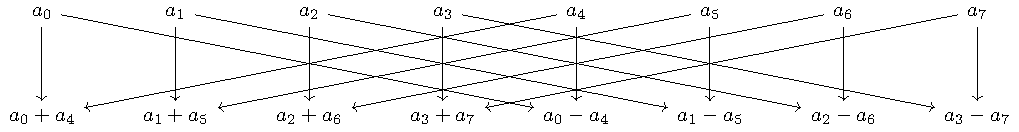
\includegraphics[width=0.8\textwidth]{figures/compiled/tikzcd1.pdf} 
        \end{center}
        \item There are in fact four repeatitions of the same butterflies:
        \begin{center}
            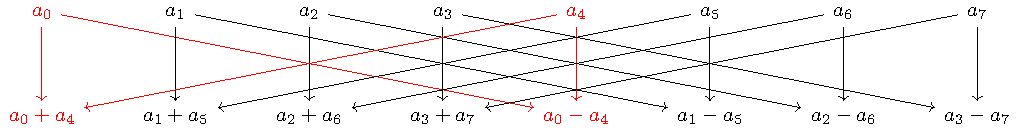
\includegraphics[width=0.8\textwidth]{figures/compiled/tikzcd2.pdf} 
        \end{center}
    \end{itemize}
\end{frame}




\begin{frame}
    \begin{itemize}
        \item After implementing the first layer, we now focus on the second layer:
        \begin{align*}
            &\mathbb{Z}_{17}[x]/(x^{4}-1) \times \mathbb{Z}_{17}[x]/(x^{4}+1)\\
            &\quad\underbrace{\cong}_{(2)}\mathbb{Z}_{17}[x]/(x^{2}-1) \times \mathbb{Z}_{17}[x]/(x^{2}+1) \times \mathbb{Z}_{17}[x]/(x^{2}-4) \times \mathbb{Z}_{17}[x]/(x^{2}+4).
        \end{align*}
        \item Our array is now the output of the above layer (layer 1), we reset the symbols:
        \[ [a_{0}, a_{1}, a_{2}, a_{3}, a_{4}, a_{5}, a_{6}, a_{7}] \]
        which denotes \( a_{0} + a_{1}x + a_{2}x^{2} + a_{3}x^{3} \) and \(a_{4} + a_{5}x + a_{6}x^{2} + a_{7}x^{3}\) in the respective space.

        \item It will project two polynomials to four polynomials:
        \begin{align*}
            a_{0} + a_{2} + (a_{1} + a_{3})x &\in \mathbb{Z}_{17}[x]/(x^{2} - 1),\\
            a_{0} - a_{2} + (a_{1} - a_{3})x &\in \mathbb{Z}_{17}[x]/(x^{2} + 1),\\
            a_{4} + 4a_{6} + (a_{5} + 4a_{7})x &\in \mathbb{Z}_{17}[x]/(x^{2} - 4),\\
            a_{4} - 4a_{6} + (a_{5} - 4a_{7})x &\in \mathbb{Z}_{17}[x]/(x^{2} + 4).
        \end{align*}
        \item In our array representation, the projection is to perform:
        \[ 
        [a_{0}, a_{1}, a_{2}, a_{3}, a_{4}, a_{5}, a_{6}, a_{7}] \mapsto [a_{0} + a_{2}, a_{1} + a_{3}, a_{0} - a_{2}, a_{1} - a_{3}, a_{4} + 4a_{6}, a_{5} + 4a_{7}, a_{4} - 4a_{6}, a_{5} - 4a_{7}].
        \]

    \end{itemize}
\end{frame}


\begin{frame}
    \begin{itemize}
        \item In our array representation, the projection is to perform:
        \[ 
            [a_{0}, a_{1}, a_{2}, a_{3}, a_{4}, a_{5}, a_{6}, a_{7}] \mapsto [a_{0} + a_{2}, a_{1} + a_{3}, a_{0} - a_{2}, a_{1} - a_{3}, a_{4} + 4a_{6}, a_{5} + 4a_{7}, a_{4} - 4a_{6}, a_{5} - 4a_{7}].
        \]
    
        The pattern is not obvious, lets make a graph: 
        \begin{center}
            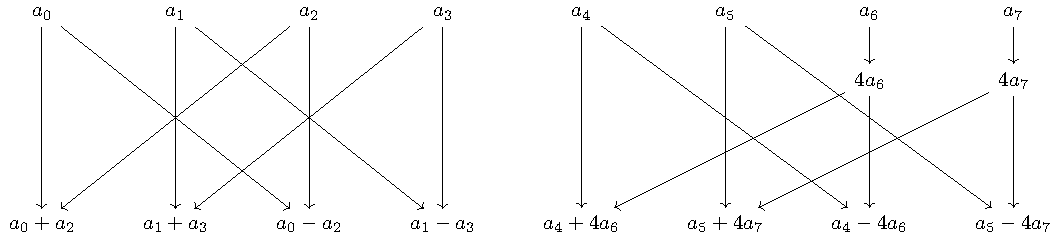
\includegraphics[width=0.8\textwidth]{figures/compiled/tikzcd3.pdf}
        \end{center}

    \end{itemize}
\end{frame}

\begin{frame}
    \begin{itemize}
        \item After implementing the second layer, we now focus on the last layer:
        \begin{align*}
            &\mathbb{Z}_{17}[x]/(x^{2}-1) \times \mathbb{Z}_{17}[x]/(x^{2}+1) \times \mathbb{Z}_{17}[x]/(x^{2}-4) \times \mathbb{Z}_{17}[x]/(x^{2}+4)\\
            &\underbrace{\cong}_{(3)} \mathbb{Z}_{17}[x]/(x-1) \times \mathbb{Z}_{17}[x]/(x+1) \times \mathbb{Z}_{17}[x]/(x-4) \times \mathbb{Z}_{17}[x]/(x+4) \\
            &\hspace{1cm} \times \mathbb{Z}_{17}[x]/(x-2) \times \mathbb{Z}_{17}[x]/(x+2) \times \mathbb{Z}_{17}[x]/(x-8) \times \mathbb{Z}_{17}[x]/(x+8).
        \end{align*}
        \item Our array is now the output of the above layer (layer 2), we reset the symbols:
        \[ [a_{0}, a_{1}, a_{2}, a_{3}, a_{4}, a_{5}, a_{6}, a_{7}] \]


        \item It will project four polynomials to eight scalars:
        \begin{align*}
            a_{0} + a_{1} &\in \mathbb{Z}_{17}[x]/(x - 1),&
            a_{0} - a_{1} &\in \mathbb{Z}_{17}[x]/(x + 1),\\
            a_{2} + 4a_{3} &\in \mathbb{Z}_{17}[x]/(x - 4),&
            a_{2} - 4a_{3} &\in \mathbb{Z}_{17}[x]/(x + 4),\\
            a_{4} + 2a_{5} &\in \mathbb{Z}_{17}[x]/(x - 2),&
            a_{4} - 2a_{5} &\in \mathbb{Z}_{17}[x]/(x + 2),\\
            a_{6} + 8a_{7} &\in \mathbb{Z}_{17}[x]/(x - 8),&
            a_{6} - 8a_{7} &\in \mathbb{Z}_{17}[x]/(x + 8).
        \end{align*}
        \item In our array representation, the projection is to perform:
        \[ 
        [a_{0}, a_{1}, a_{2}, a_{3}, a_{4}, a_{5}, a_{6}, a_{7}] \mapsto 
        [a_{0} + a_{1}, a_{0} - a_{1}, a_{2} + 4a_{3}, a_{2} - 4a_{3}, a_{4} + 2a_{5}, a_{4} - 2a_{5}, a_{6} + 8a_{7}, a_{6} - 8a_{7}].
        \]


    \end{itemize}
\end{frame}

\begin{frame}
    \begin{itemize}
        \item In our array representation, the projection is to perform:
        \[ 
        [a_{0}, a_{1}, a_{2}, a_{3}, a_{4}, a_{5}, a_{6}, a_{7}] \mapsto 
        [a_{0} + a_{1}, a_{0} - a_{1}, a_{2} + 4a_{3}, a_{2} - 4a_{3}, a_{4} + 2a_{5}, a_{4} - 2a_{5}, a_{6} + 8a_{7}, a_{6} - 8a_{7}].
        \]
    
        The pattern is not obvious, lets make a graph: 
        \begin{center}
            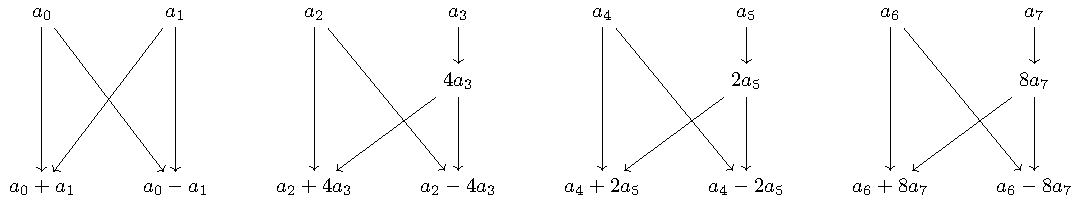
\includegraphics[width=0.8\textwidth]{figures/compiled/tikzcd4.pdf}
        \end{center}
        

    \end{itemize}
\end{frame}

\begin{frame}
    In total, the projection can be represented by the following graph:
    \begin{center}
        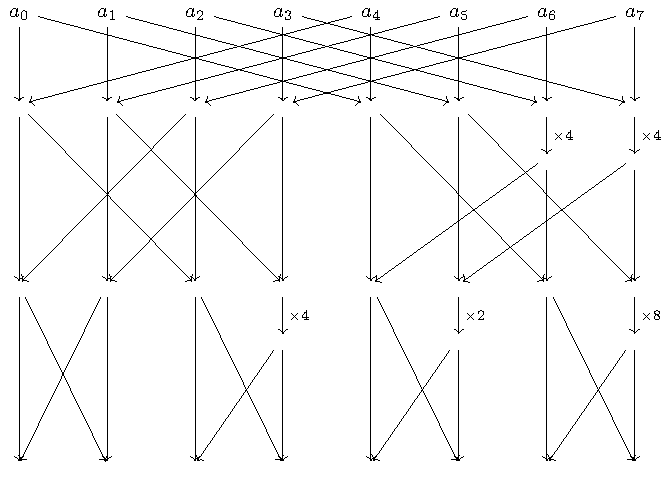
\includegraphics[width=0.7\textwidth]{figures/compiled/tikzcd5.pdf}
    \end{center}
\end{frame}

\begin{frame}
    \begin{itemize}
        \item Ok! After the projection, the point-wise multiplication is simple. 
        \item The remark I want to make here is that, during the whole process, the multiplication is performed modulo \( 17 \). 
        Such modulus multiplication (mod-mul for short) is a time-consuming operation.
        \item To deal with this, mathematicians invented various \emph{reduction algorithms}, e.g., Barrett reduction, Montgomery reduction, Plantard reduction etc.
        \item The choice of reduction algorithm depends on many factors, including the machine architecture, the parallelization, etc.
        \item There is a review in the following paper:

    \end{itemize}
\end{frame}

\begin{frame}
\begin{itemize}
    \item Finally, we have to rebuild the polynomial from the output of the last layer.
    \item Note that the rebuiding is the inverse of the projection, so we can rebuild the polynomial according to the graph, but you should look it conversely:
    \begin{center}
        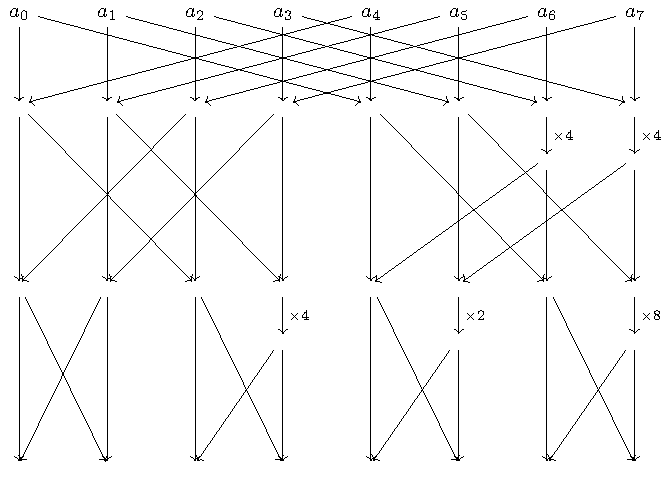
\includegraphics[width=0.6\textwidth]{figures/compiled/tikzcd5.pdf}
    \end{center}
\end{itemize}
\end{frame}





\begin{frame}[allowframebreaks]{References}
    \printbibliography
\end{frame}

\end{document}
